\begin{titre}[Informations chiffrées]

\Titre{Évolutions successives}{4}
\end{titre}


\begin{CpsCol}
\begin{description}
\item[$\square$] Exploiter la relation entre deux valeurs successives et leur taux d'évolution.
\item[$\square$] Calculer le taux d'évolution global à partir des taux d'évolution successifs. Calculer un taux d'évolution réciproque.
\end{description}
\end{CpsCol}

 

\begin{DefT}{Évolutions successives}\index{Évolutions! successives}
Lorsqu'une quantité subit des évolutions successives $t_1$, $t_2$, $t_3$, ...de sa valeur initiale, cette quantité subit une évolution globale $t$.
\end{DefT}

\begin{Ex}
 Chaque année, le prix de l'électricité en France augmente d'un certain pourcentage. Le prix de l'électricité a augmenté de 5,9\% le 1er juin 2019 et il avait augmenté de  2,8\% le 1er juin 2018.
\end{Ex}

\begin{ThT}{Taux global d'évolution}
Le taux global d'évolution correspondant à deux évolutions successives de taux respectifs $t_1$ et $t_2$  est le réel $t$ tel que $1+t = \left(1+t_1\right)\left(1+ t_2 \right)$.
\end{ThT}


\begin{Ex}
Dans l'exemple précédent, le prix de l'électricité a augmenté de 5,9\% le 1er juin 2019 et augmenté de  2,8\% le 1er juin 2018.

$t_1=5,9\%=\frac{5,9}{100}$ et $t_2=2,8\%=\frac{2,8}{100}$

donc $1+t = \left(1+\frac{2,8}{100}\right)\left(1+ \frac{5,9}{100} \right)$.
 
$1+t = 1,028 \times 1,059 \approx 1,088$ donc $t = 1,088 - 1 \approx 0,088$ ou $t \approx \frac{8,8}{100}$ ou aussi, $t\approx 8,8\%$.
\end{Ex}




\begin{Rq}
On peut faire correspondre un coefficient multiplicateur global, $CM_g$, au taux global d'évolution tel que $$CM = \left(1+t_1\right)\left(1+t_2\right)$$
\end{Rq}


\begin{Ex}
Un objet A coute 75 euros initialement en 2015. En 2016, cet objet a augmenté de 5\% et son prix a baissé en 2017 de 4\%. Le coefficient multiplicateur global est donc $CM = \left(1+\frac{5}{100}\right)\left(1-\frac{4}{100}\right)=1,05 \times 0,96 = 1,008$.\\
Le taux de pourcentage est donc égal à $0,008 \times 100 = 0,8$. Sur les 2 années, l'objet a augmenté de 0,8\%. 
\end{Ex}


\begin{Dem}
Soit deux taux respectifs $t_1$ et $t_2$. On appelle $CM_1 = 1+t_1$ et $CM_2 = 1+t_2$.\\
Soit $P_0$ la valeur initiale. Après la première évolution, $P_1=CM_1 \times P_0 = \left(1+t_1\right)\times P_0 $\\
Après la seconde évolution, $P_2=CM_2 \times P_1 = CM_2 \times CM_1 \times P_0 =\left(1+t_2\right)\times \left(1+t_1 \right)\times P_0 $.\\
Après les 2 évolutions, $P_2=\left(1+t_2\right)\times \left(1+t_1\right)\times P_0 $. Donc Le coefficient multiplicateur global est $CM = \left(1+t_1\right)\left(1+t_2\right)$.
\end{Dem}

\begin{ThT}{Taux global d'évolution pour $n$ évolutions}
Le taux global d'évolution correspondant à $n$ évolutions successives de taux respectifs $t_1$, $t_2$, $t_3$, ..., $t_n$ est le réel $t$ tel que $$1+t = \left(1+t_1\right)\left(1+t_2\right)\left(1+t_3\right)\cdots \left(1+t_n\right)$$
\end{ThT}

\begin{Rq}
On peut faire correspondre un coefficient multiplicateur global, $CM_g$, au taux global d'évolution tel que $$CM = \left(1+t_1\right) \left(1+t_2\right)\left(1+t_3\right)\cdots \left(1+t_n\right)$$
\end{Rq}

\begin{Ex}
Un article subit les évolutions suivantes lors des 3 dernières années : 3\% en 2015, $-1$\% en 2016 et 2\% en 2017. Quel est le taux global d'évolution sur ces 3 années ?

Le taux d'évolution global est : $CM_g=(1+0,03)(1-0,01)(1+0,02)=1,03 \times 0,99 \times 1,02 = 1,04$ arrondi à 0,01 près.

On peut donc dire que sur les 3 dernières années, l'article a augmenté de 4\%.
\end{Ex}



\mini{
\EPC{1}{IC-34}{Chercher.}

%\EPC{1}{IC-16}{Chercher.}
\EPC{1}{IC-36}{Chercher.}


\EPC{0}{IC-5}{Chercher.}
}{
\EPC{1}{IC-33}{Chercher.}

\EPC{1}{IC-3}{Chercher.}
}


\EPC{0}{IC-9}{Chercher.}




\begin{DefT}{Évolution réciproque}\index{Évolution! réciproque}
Une quantité non nulle $V_i$ subit une évolution de taux $t$ et devient égale à une quantité $V_f$. 

Le \textbf{taux réciproque} de $t$ est le taux d'évolution $t'$ qui permet de passer de $V_f$ à $V_i$.
\end{DefT}


\begin{Ex}
\begin{minipage}{0.7\linewidth}
 
Un objet A coute 50 euros (valeur initiale). Une baisse de 20\% fait passer son prix à 40 euros(valeur finale). Le taux d'évolution $t$ est donc égal à $-20$\%.  

Le taux réciproque $t'$ est le taux qui fait passer de 40 euros (la valeur du prix finale) à 50 euros (la valeur du prix initiale). Donc $t'=\frac{50}{40}=1,25$ donc $t' =+25\%$.
\end{minipage}
\begin{minipage}{0.4\linewidth}
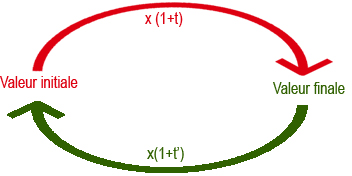
\includegraphics[scale=0.5]{taux_reciproque.jpg} 
\end{minipage}

\end{Ex}


\begin{ThT}{Taux d'évolution réciproque}
\begin{minipage}{0.74\linewidth}
 Le coefficient multiplicateur réciproque $CM'$ associe à l'évolution réciproque $t'$ est l'inverse du coefficient multiplicateur non nul $CM$ associé à l'évolution de départ $t$. 
 
 On a : $CM' = \frac{1}{CM}$ c'est à dire : $CM \times CM' = 1$ 

\end{minipage}
\hfill
\begin{minipage}{0.25\linewidth}

\includegraphics[scale=0.5]{taux_reciproque2.png} 
\end{minipage}
\end{ThT}

\ROC





\begin{Rq}
Le taux réciproque $t'$ n'est pas égal au taux initial $t'$.
\end{Rq}
 


\mini{
\EPC{1}{IC-39}{Chercher.}

\EPC{1}{IC-7}{Chercher.}

\EPCP{1}{IC-40}{Chercher.}
}{
\EPC{1}{IC-35}{Chercher.}

\EPC{0}{IC-37}{Chercher.}
 
\EPC{1}{IC-38}{Chercher.} 
}
 
 